\begin{tikzpicture}[scale=0.85]
\begin{axis}[xmax=3,ymax=1,ymin=0,grid=major,
xlabel={T},
ylabel={|M|},
extra x ticks={2.267},
extra x tick labels={$T_c$}]
\begin{scope}
\addplot[mark=+,mark options={black}, white]coordinates{(1.75,0.1)};\label{plot:mcB}
\addplot[mark=+,mark options={white}, white]coordinates{(1.75,0.1)};
\end{scope}
\only<1-2>{\addplot[mark=o,mark options=blue,white] coordinates {
(1.00,1)
(1.20,1)
(1.40,0.99)
(1.60,0.98)
(1.70,0.97)
(1.80,0.957)
(1.90,0.937)
(2.00,0.91)
(2.05,0.89)
(2.10,0.87)
(2.15,0.84)
(2.20,0.783)
(2.225,0.74)
(2.25,0.67)
(2.2692,0.54)
(2.275,0.48)
(2.30,0.39)
(2.35,0.20)
(2.40,0.13)
(2.45,0.10)
(2.50,0.08)
(2.60,0.045)
(2.70,0.03)
(2.80,0.027)
(2.90,0.026)
(3.00,0.025)};\label{plot:mc}}
\only<2>{\addplot[mark=+,mark options={black}, white] coordinates {
(1.00,1)
(1.20,1)
(1.40,0.99)
(1.60,0.98)
(1.70,0.97)
(1.80,0.957)
(1.90,0.938)
(2.00,0.907)
(2.05,0.893)
(2.10,0.871)
(2.15,0.84)
(2.20,0.784)
(2.225,0.745)
(2.25,0.687)
(2.2692,0.62)
(2.275,0.585)
(2.30,0.493)
(2.35,0.303)
(2.40,0.213)
(2.45,0.152)
(2.50,0.126)
(2.60,0.100)
(2.70,0.07)
(2.80,0.068)
(2.90,0.06)
(3.00,0.05)};}
\only<2-1>{\addplot[mark=triangle,mark options={black}, white] coordinates {
(2.3,0.730)
(2.3,0.638)
(2.3,0.589)
(2.3,0.537)
(2.3,0.483)
(2.3,0.449)
(2.3,0.413)
(2.3,0.390)
(2.3,0.357)
(2.3,0.318)
(2.3,0.362)
(2.3,0.242)
};}
\addplot[line width=1pt,red,samples = 500,domain=1.001:5]
	{(1-sinh(2/(x))^(-4))^(0.125)};\label{plot:analytical}
\addplot[red,line width= 1pt] coordinates {(2.267,0.55)(2.267,0)(3,0)};


\end{axis}
\end{tikzpicture}